\documentclass[border=2mm]{standalone}
\usepackage{pgfplots}
\usepackage{tikz}

\begin{document}

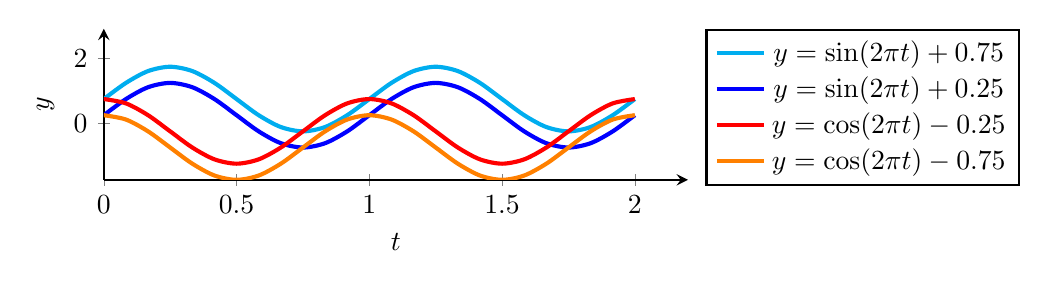
\begin{tikzpicture}
    \begin{axis}[
        axis lines=left,
        enlargelimits=upper,
        domain=0:2,
        legend pos=outer north east,
        width=9cm,
        height=3.5cm,
        thick,
        xlabel=$t$,
        ylabel=$y$,
        ymax=2.5,
        legend entries = {
            $y=\sin(2\pi t)+0.75$,
            $y=\sin(2\pi t)+0.25$,
            $y=\cos(2\pi t)-0.25$,
            $y=\cos(2\pi t)-0.75$
        }
    ]
        \addplot [smooth, color=cyan, line width=1.5] {sin(deg(2*pi*x))+0.75};
        \addplot [smooth, color=blue, line width=1.5] {sin(deg(2*pi*x))+0.25}; 
        \addplot [smooth, color=red, line width=1.5] {cos(deg(2*pi*x))-0.25}; 
        \addplot [smooth, color=orange, line width=1.5] {cos(deg(2*pi*x))-0.75};
    \end{axis}
\end{tikzpicture}

\end{document}
